\documentclass[14pt]{beamer}
\usetheme{Montpellier}
\usepackage[utf8]{inputenc}
\usepackage[english]{babel}
\usepackage{amsmath}
\usepackage{amsfonts}
\usepackage{amssymb}
\usepackage{graphicx}
\usepackage{enumitem}

\author{Oumaima Al Qoh, Francisco Arrieta, Lucia Camenisch, Manuela Giansante, Emily Schmidt, Camille Beatrice Valera}
\title{Case Study B \\ Pain Relief Medication}
\date{April 28, 2023} 
%\subject{}
%\logo{}
%\institute{}

  
\setbeamertemplate{navigation symbols}{
\usebeamerfont{footline}
\insertframenumber / \inserttotalframenumber
}



\begin{document}


\begin{frame}
\titlepage
\end{frame}



\begin{frame}
\frametitle{Table of contents}
\tableofcontents
\end{frame}


\section{Objectives}
\begin{frame}
\frametitle{First objective}
\textit{Determine the minimum dosage amount of the drugs that achieves \textbf{efficacy}.}

\bigskip

The dosage of a drug is said to be \textbf{efficient} if at least 50\% of the subjects are responding.
\end{frame}


\begin{frame}
\frametitle{Second objective}
\textit{Detect whether a \textbf{synergy} exists between the two drugs.}

\bigskip

If the combined efficacy of the two drug dosages is greater than the sum of the individual efficacy of each drug for its respective dosage, there is \textbf{synergy}.
\end{frame}


\section{Identifying synergy using the method of isoboles}
\begin{frame}
\frametitle{Identifying synergy with the isoboles method}
The isoboles method is a graphical representation which allows to identify synergy and helps to better understand the concept.
\end{frame}

\begin{frame}
\begin{center}
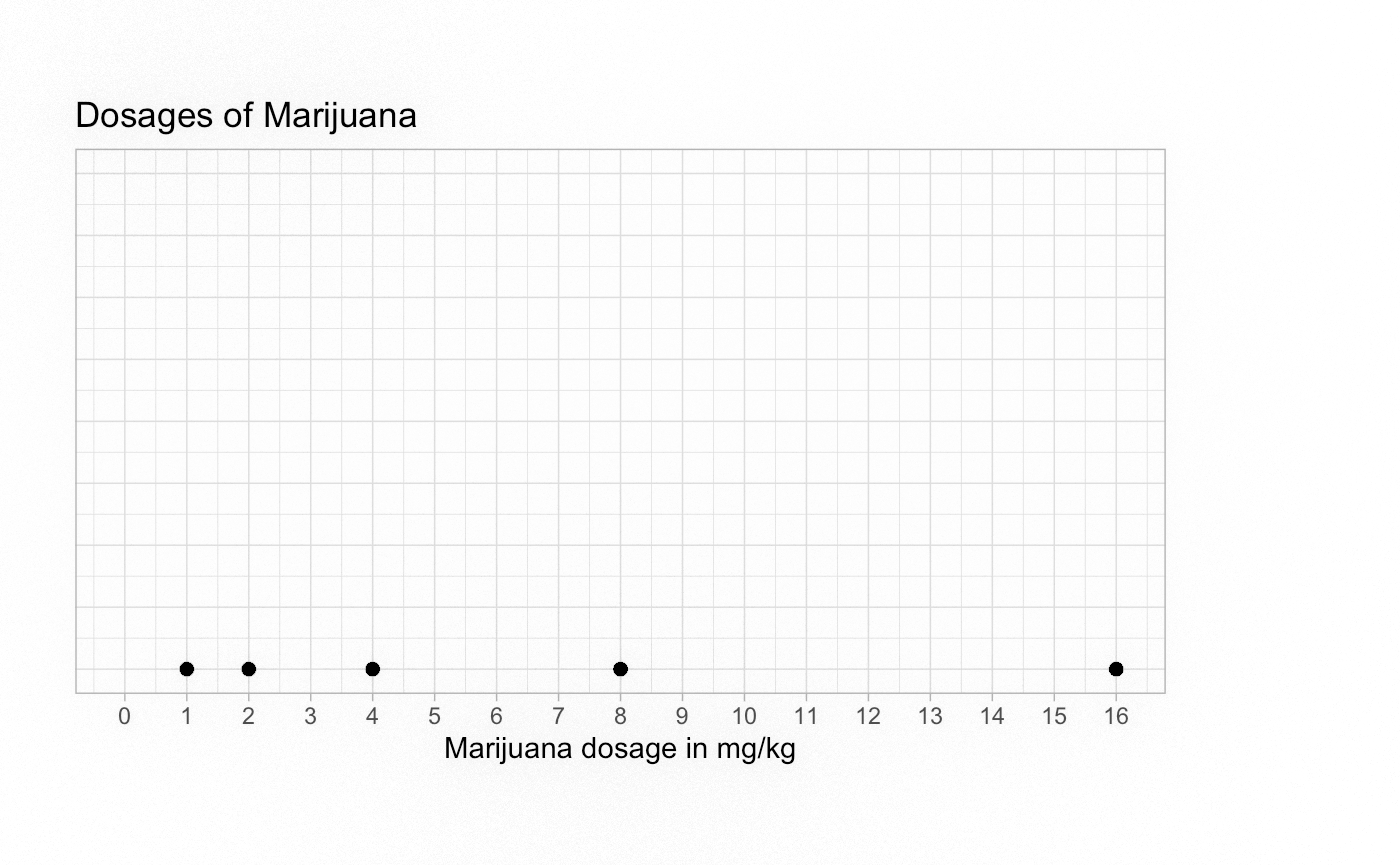
\includegraphics[scale=0.24]{img1.png}
\end{center}
\end{frame}

\begin{frame}
\begin{center}
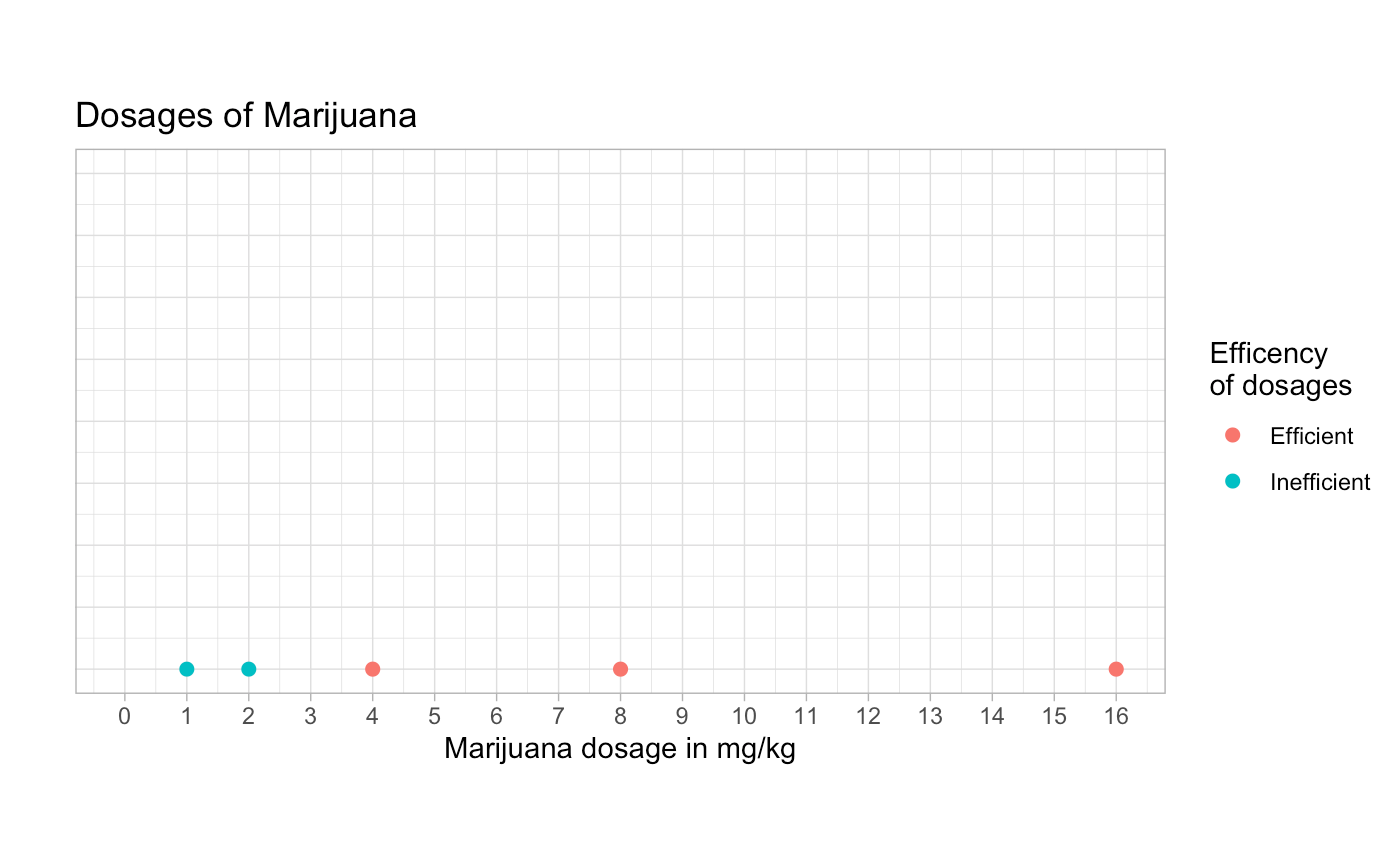
\includegraphics[scale=0.24]{img2.png}
\end{center}
\end{frame}

\begin{frame}
\begin{center}
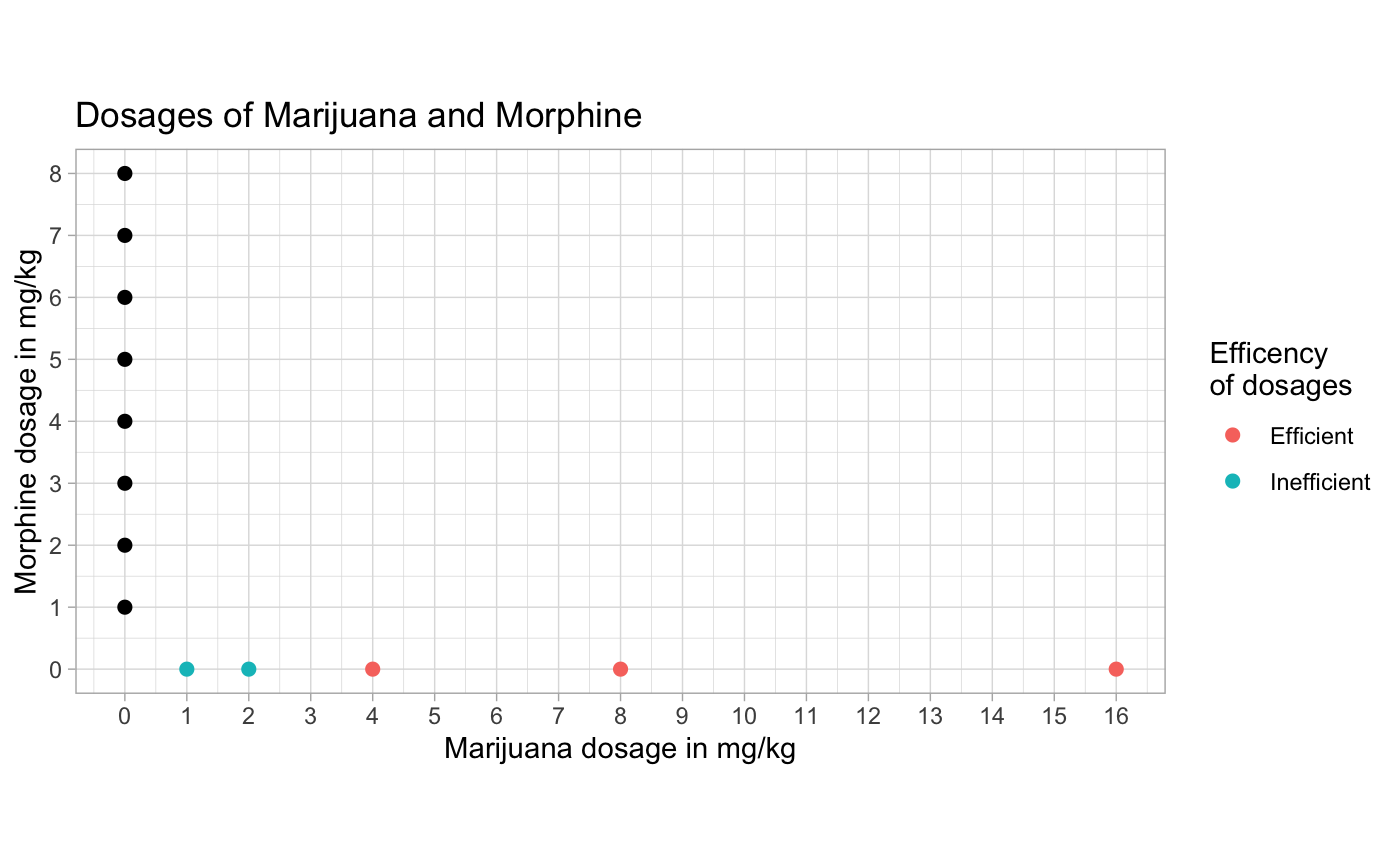
\includegraphics[scale=0.24]{img3.png}
\end{center}
\end{frame}

\begin{frame}
\begin{center}
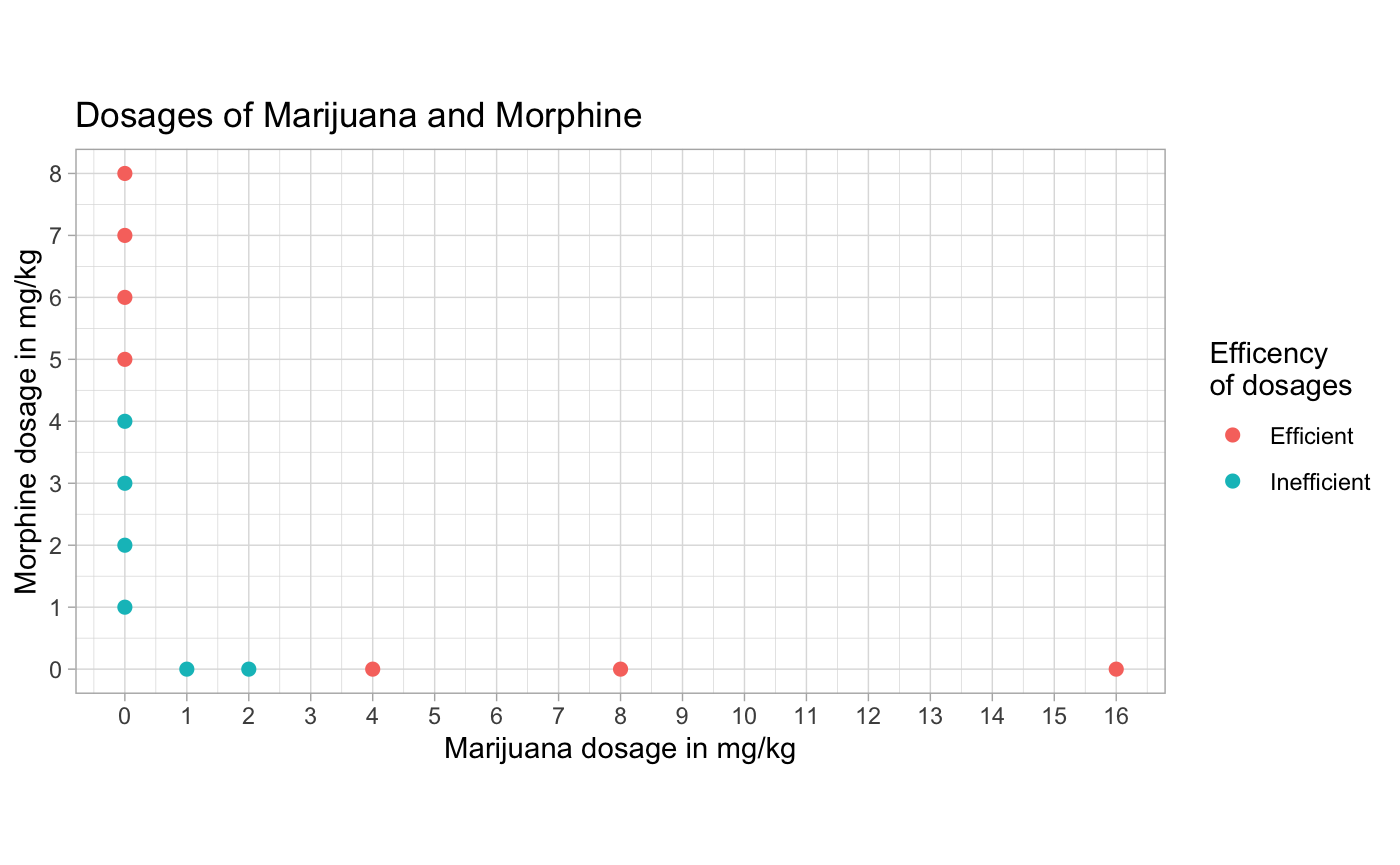
\includegraphics[scale=0.24]{img4.png}
\end{center}
\end{frame}

\begin{frame}
\begin{center}
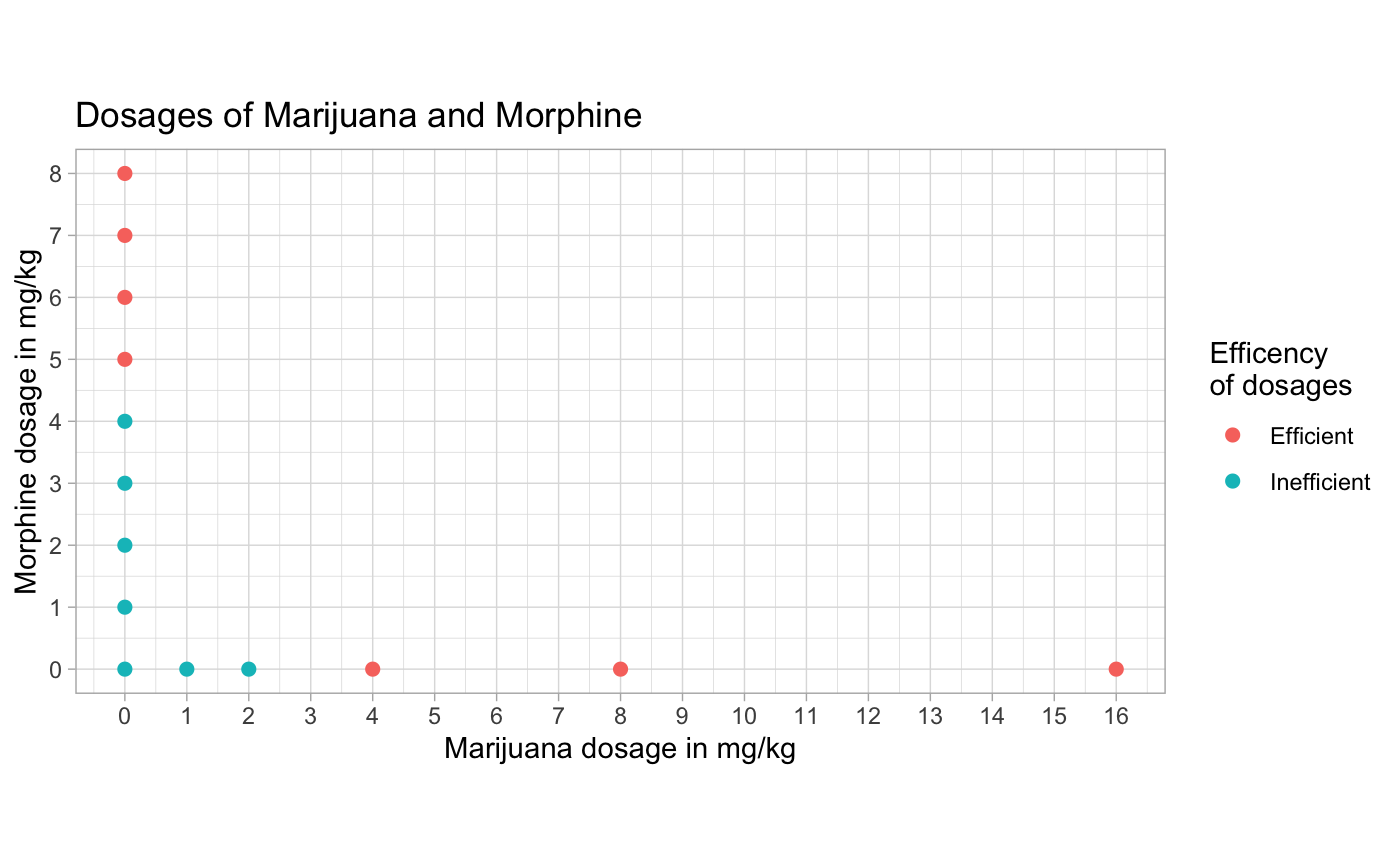
\includegraphics[scale=0.24]{img5.png}
\end{center}
\end{frame}

\begin{frame}
\begin{center}
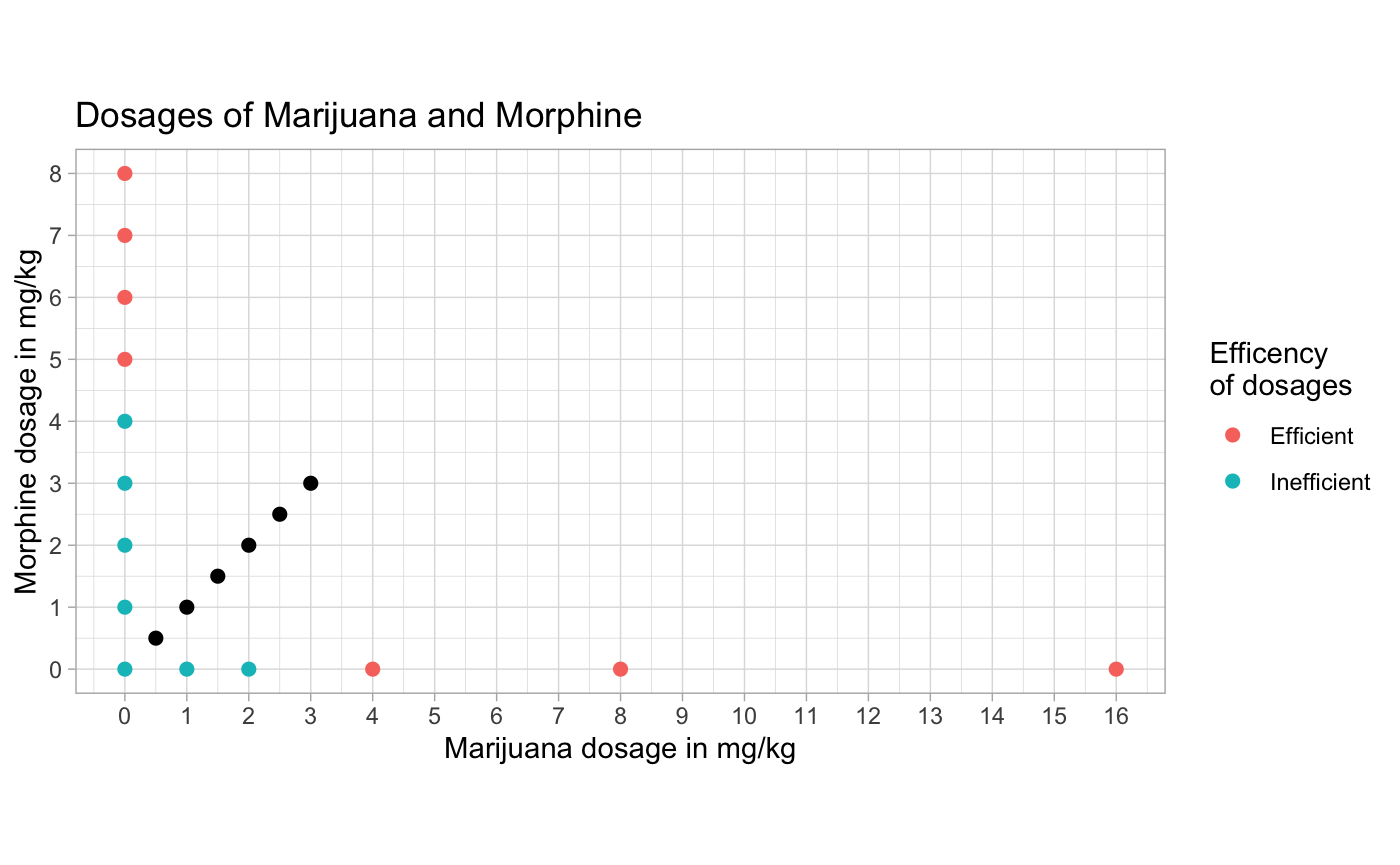
\includegraphics[scale=0.24]{img6.png}
\end{center}
\end{frame}

\begin{frame}
\begin{center}
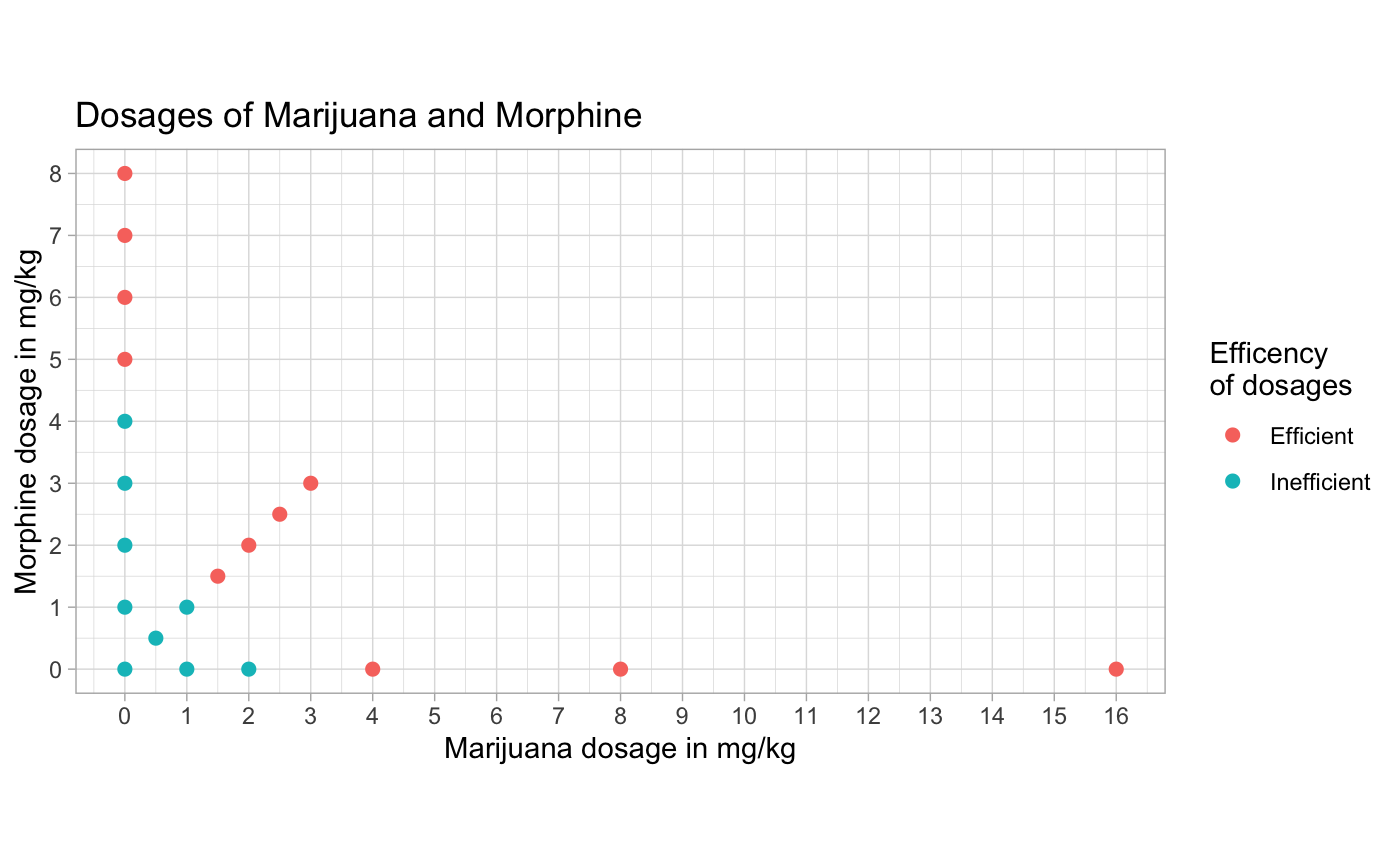
\includegraphics[scale=0.24]{img7.png}
\end{center}
\end{frame}

\begin{frame}
\begin{center}
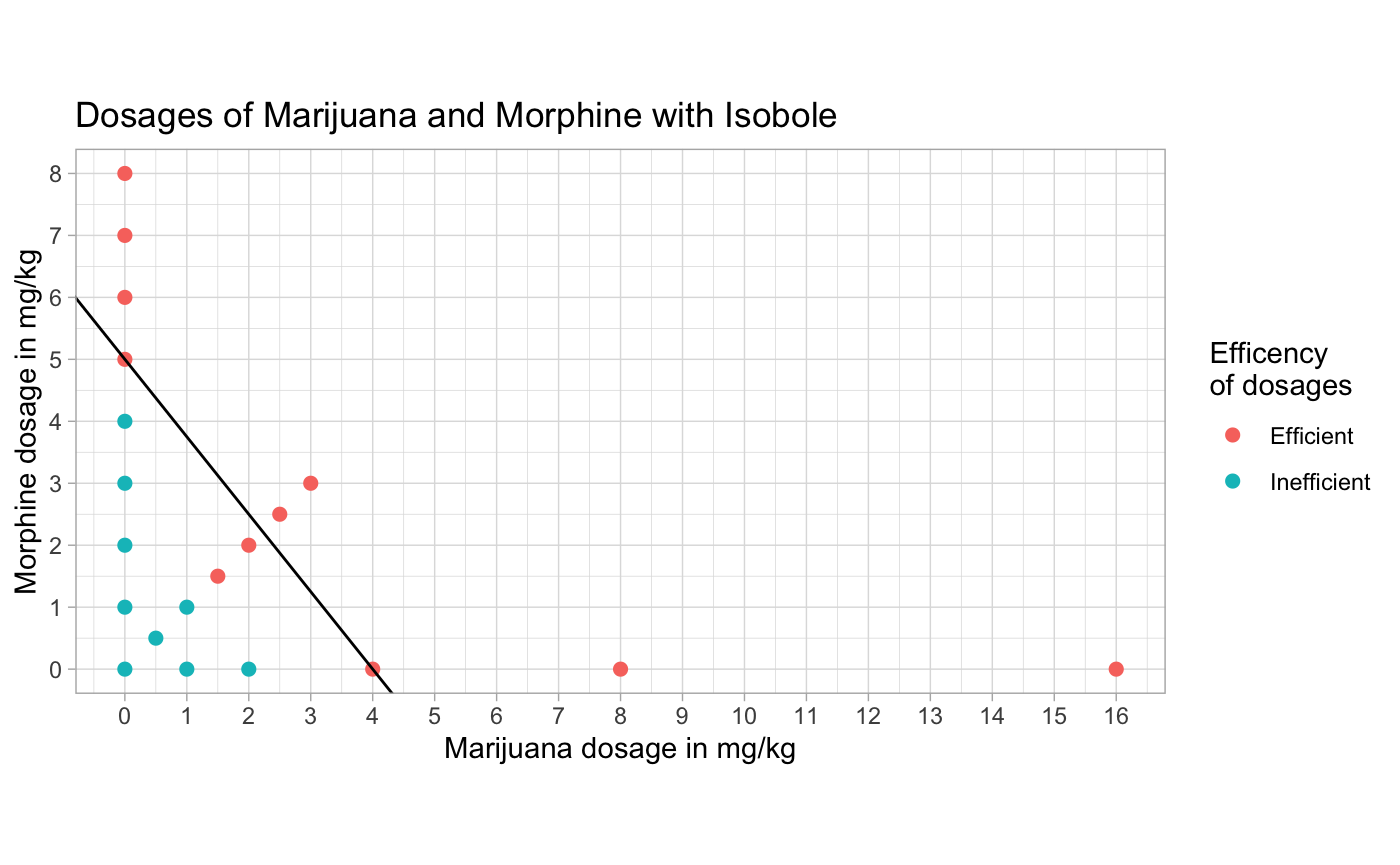
\includegraphics[scale=0.24]{img8.png}
\end{center}
\end{frame}

\section{Isobole insights}
\begin{frame}
\frametitle{Isobole insights}
\begin{itemize}[label={$\blacktriangleright$}]
\item Using 4 mg/kg of marijuana gives an equivalent effect ($\geq$ 50\% of mice responding) to using 5 mg/kg of morphine.
\item Combined dosages of the two drugs which are on the isobole have an equivalent effect to the ones mentioned above.
\item A combined dosage which is under the isobole but is still efficient is synergic.
\end{itemize}
\end{frame}

\section{Isobole conclusion}
\begin{frame}
\frametitle{Isobole conclusion}
\begin{itemize}[label={\checkmark}]
\item \textbf{First objective, minimal efficient dosage:} \\
\begin{itemize}[label={$\blacktriangleright$}]
\item 4.0 mg/kg for marijuana alone;
\item 5.0 mg/kg for morphine alone;
\item 1.5 mg/kg of each for both drugs.
\end{itemize}
\item \textbf{Second objective, synergy:} \\
Dosages of 1.5 mg/kg and 2.0 mg/kg each are synergic.
\end{itemize}
\end{frame}

\section{Isoboles method assumption}
\begin{frame}
\frametitle{Isoboles method assumption}
The ratio between dosages of morphine and marijuana when they give the same efficiency level is constant.
\end{frame}

\begin{frame}
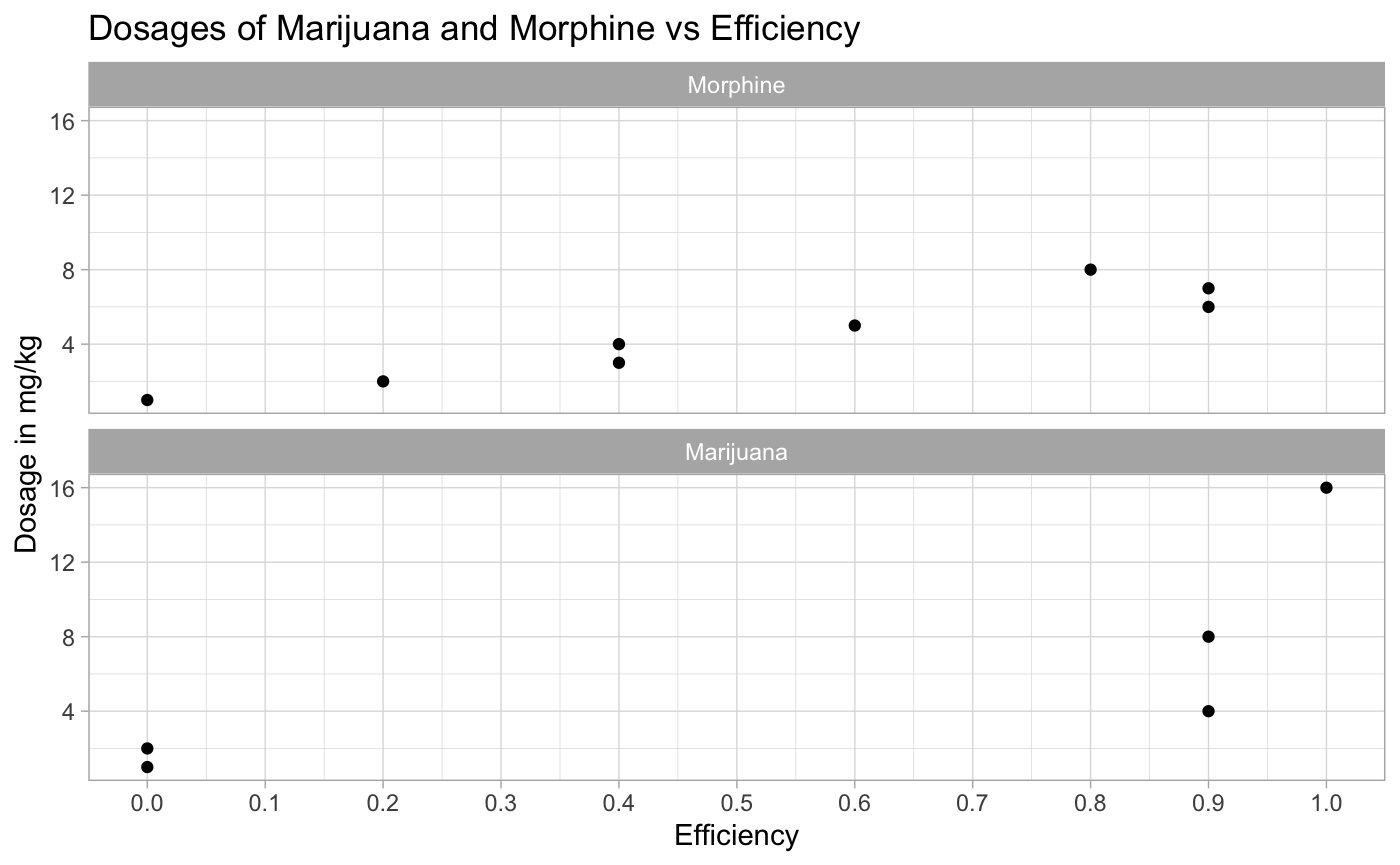
\includegraphics[scale=0.22]{dos_vs_eff.png}
\end{frame}

\begin{frame}
\begin{itemize}[label={$\blacktriangleright$}]
\item Only two common efficiency levels, 0.0 and 0.9
\item This is not enough to verify the assumption for this experiment.
\item This weakness is due to dosage choices for marijuana.
\item However, the linear isobole method is used in multiple experiments which are extremely similar.
\end{itemize}
\end{frame}
\end{document}